\documentclass[tikz,border=8pt]{standalone}
\usepackage{pifont}
\usetikzlibrary{positioning,calc,arrows.meta,shapes.geometric}
\definecolor{accB}{HTML}{1769AA}
\definecolor{fillB}{HTML}{DCEAF5}
\definecolor{accO}{HTML}{C85A00}
\definecolor{fillO}{HTML}{FCE8D5}
\definecolor{accP}{HTML}{6B46A1}
\definecolor{fillP}{HTML}{E9DDF3}
\definecolor{ink}{HTML}{18212B}
\definecolor{slate}{HTML}{66727D}
\definecolor{chipgray}{HTML}{D9DEE3}
\definecolor{chipdark}{HTML}{5B6773}
\newcommand{\frozenmark}{\textcolor{slate}{\ding{100}}}
\begin{document}
\begin{tikzpicture}[
  font=\small, ink/.style={draw=ink, thick},
  tok/.style={draw=ink, minimum size=4.2mm, inner sep=0pt},
  gtok/.style={tok, fill=chipgray},
  htok/.style={tok, draw=accP, very thick, fill=fillP},
  ctok/.style={tok, fill=chipdark},
  rtok/.style={tok, fill=white},
  gate/.style={draw=ink, minimum size=2.6mm, inner sep=0pt, font=\scriptsize},
  arr/.style={-{Stealth[length=2mm]}, ink},
  tarr/.style={-{Stealth[length=2.2mm]}, accP, very thick},
  lbl/.style={font=\small, text=ink},
]

%%%%%%%%%%%%%%%%%%%%%%%%%%%%%%%%%%%%%%%%%%%%%%%%%%%%%%%%%%%%%%
%% Panel (a): HGKV cross-section
%%%%%%%%%%%%%%%%%%%%%%%%%%%%%%%%%%%%%%%%%%%%%%%%%%%%%%%%%%%%%%
\begin{scope}[shift={(0,-1.05)}]
  % token row
  \foreach \i in {0,...,3} \node[gtok] (t\i) at (0.46*\i, 0) {};
  \foreach \i in {4,...,6} \node[htok] (t\i) at (0.46*\i, 0) {};
  \foreach \i in {7,...,9} \node[ctok] (t\i) at (0.46*\i, 0) {};
  \foreach \i in {10,...,11} \node[rtok] (t\i) at (0.46*\i, 0) {};
  % group labels under gate row
  % gate strip
  \foreach \i in {0,...,3}  \node[gate] (g\i) at (0.46*\i, -0.52) {\scriptsize 0};
  \foreach \i in {4,...,6}  \node[gate, draw=accP, text=accP] (g\i) at (0.46*\i, -0.52) {\scriptsize 1};
  \foreach \i in {7,...,11} \node[gate] (g\i) at (0.46*\i, -0.52) {\scriptsize 0};
  \node[lbl, anchor=east] at (-0.35, -0.52) {gate $g$};
  % group braces / labels
  \node[lbl, anchor=north, align=center, font=\scriptsize] at (0.69, -0.95) {task +\\summaries};
  \node[lbl, anchor=north, align=center, font=\scriptsize, text=accP] at (2.30, -0.95) {restored\\history img};
  \node[lbl, anchor=north, align=center, font=\scriptsize] at (3.68, -0.95) {current\\screen};
  \node[lbl, anchor=north, align=center, font=\scriptsize] at (4.83, -0.95) {resp.};
  % attention block
  \node[ink, rounded corners=2pt, minimum width=6.4cm, minimum height=1.05cm,
        anchor=south west] (attn) at (-0.35, 1.55)
        {self-attention, last 8 layers\; \frozenmark};
  % frozen up-arrows
  \foreach \i in {1,8,10} \draw[arr] (t\i.north) -- (t\i.north |- attn.south);
  % delta box on the teal path
  \node[draw=accP, very thick, rounded corners=2pt, fill=fillP, font=\small,
        minimum height=5.2mm] (dkv) at (2.30, 0.95) {$\Delta K,\Delta V$ (low-rank)};
  \draw[tarr] (t5.north) -- (dkv.south);
  \draw[tarr] (dkv.north) -- (dkv.north |- attn.south);
  \node[lbl, text=accP, font=\scriptsize, anchor=west] at ($(dkv.east)+(0.05,0.22)$) {$\times\, g$};
  % bypass note
  \node[lbl, font=\scriptsize, anchor=north west, align=left] at (-0.35, -1.75)
    {$B{=}0 \Rightarrow g\equiv 0 \Rightarrow$ bitwise-exact frozen policy
     \quad\frozenmark\,$=$ frozen};
  % panel tag
  \node[lbl, font=\small\bfseries, anchor=south west] at (-0.35, 2.75) {(a) \textsc{hgkv}: gated K/V interface};
\end{scope}

%%%%%%%%%%%%%%%%%%%%%%%%%%%%%%%%%%%%%%%%%%%%%%%%%%%%%%%%%%%%%%
%% Panel (b): proposal-conditioned pass-2
%%%%%%%%%%%%%%%%%%%%%%%%%%%%%%%%%%%%%%%%%%%%%%%%%%%%%%%%%%%%%%
\begin{scope}[shift={(8.6,2.35)}]
  \tikzset{chip/.style={draw=ink, minimum size=2.6mm, inner sep=0pt},
           chipB/.style={chip, draw=accB, very thick, fill=fillB},
           chipO/.style={chip, draw=accO, very thick, fill=fillO}}
  % prompt A: recent-B allocation
  \node[ink, rounded corners=2pt, inner sep=3pt] (pa) at (0,0) {%
    \begin{tikzpicture}[baseline]
      \foreach \i in {0,...,5} \node[chip] at (0.32*\i,0) {};
      \foreach \i in {6,...,9} \node[chipB] at (0.32*\i,0) {};
    \end{tikzpicture}};
  \node[lbl, font=\scriptsize, anchor=north] at (pa.south) {Recent-$B$};
  % policy box 1
  \node[ink, rounded corners=2pt, right=4.5mm of pa, align=center, inner sep=3pt]
    (pol1) {policy+\textcolor{accP}{\textsc{hgkv}} \frozenmark};
  \node[lbl, right=4mm of pol1] (a1) {$a_1$};
  \draw[arr] (pa) -- (pol1);
  \draw[arr] (pol1) -- (a1);
  \node[lbl, font=\scriptsize, anchor=south] at (a1.north) {proposal};

  % two-tower scorer
  \node[draw=ink, trapezium, trapezium angle=68, minimum width=1.55cm, inner sep=2pt,
        font=\scriptsize, align=center] (tw1) at (0.45,-1.75) {event feats\\$+$ witness$(a_1)$};
  \node[draw=ink, trapezium, trapezium angle=68, minimum width=1.35cm, inner sep=2pt,
        font=\scriptsize, align=center] (tw2) at (2.75,-1.75) {budget\\context};
  \node[circle, draw=ink, inner sep=1.2pt, font=\scriptsize] (dot) at (1.6,-2.45) {$\cdot$};
  \draw[arr] (tw1.south) -- (dot);
  \draw[arr] (tw2.south) -- (dot);
  \draw[arr] (a1.south) |- node[pos=0.75, above, font=\scriptsize]{witness}
    ($(tw1.north)+(0,0.28)$) -- (tw1.north);
  % score strip over full trace
  \node[ink, rounded corners=2pt, inner sep=3pt, below=4.5mm of dot] (ss) {%
    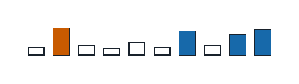
\begin{tikzpicture}[baseline]
      \foreach \i/\h in {0/0.10, 1/0.34, 2/0.12, 3/0.08, 4/0.16, 5/0.10, 6/0.30, 7/0.12, 8/0.26, 9/0.32}
        \draw[ink] (0.32*\i,-0.13) rectangle (0.32*\i+0.20,-0.13+\h);
      \fill[accO] (0.32*1,-0.13) rectangle (0.32*1+0.20,-0.13+0.34);
      \foreach \i/\h in {6/0.30, 8/0.26, 9/0.32}
        \fill[accB] (0.32*\i,-0.13) rectangle (0.32*\i+0.20,-0.13+\h);
    \end{tikzpicture}};
  \node[lbl, font=\scriptsize, anchor=west] at (ss.east) {$S^{*},\,|S^{*}|{=}B$};
  \draw[arr] (dot) -- (ss);

  % branch
  \node[lbl, font=\scriptsize, align=center, below=4mm of ss] (br) {$S^{*}$ $=$ recent tail?};
  \draw[arr] (ss) -- (br);
  \node[lbl, right=9mm of br, font=\scriptsize] (emit) {emit $a_1$};
  \draw[arr] (br) -- node[above, font=\scriptsize]{yes} (emit);
  % prompt B: displaced allocation
  \node[ink, rounded corners=2pt, inner sep=3pt, below=5mm of br, xshift=-14mm] (pb) {%
    \begin{tikzpicture}[baseline]
      \foreach \i in {0,2,3,4,5,7} \node[chip] at (0.32*\i,0) {};
      \node[chipO] at (0.32*1,0) {};
      \foreach \i in {6,8,9} \node[chipB] at (0.32*\i,0) {};
    \end{tikzpicture}};
  \draw[arr] (br) -- node[right, font=\scriptsize]{no} (pb.north);
  \node[ink, rounded corners=2pt, right=4.5mm of pb, align=center, inner sep=3pt]
    (pol2) {policy+\textcolor{accP}{\textsc{hgkv}} \frozenmark};
  \node[lbl, right=4mm of pol2] (a2) {$a_2$};
  \draw[arr] (pb) -- (pol2);
  \draw[arr] (pol2) -- (a2);
  \node[lbl, font=\scriptsize, anchor=south] at (a2.north) {final};
  \node[lbl, font=\scriptsize, anchor=north west, align=left] at ($(pb.south west)+(0,-0.25)$)
    {same weights; 2nd pass only on displacement};
  % panel tag
  \node[lbl, font=\small\bfseries, anchor=south west] at (-1.1, 0.55) {(b) proposal-conditioned re-decision};
\end{scope}
\end{tikzpicture}
\end{document}
